\chapter[Multiplanar Imaging]{Autonomous Imaging of Multiplanar Regions through
Quadcopter}
\label{ch:multiplanar}
\section{Introduction}
Consider a visit to an art gallery or ancient temples. In such scenarios, we
would like to get an unrolled view of scenes depicted on the walls so that we
get the output mosaic of the input scene as if it is present on a single plane.
We have to capture each surface orthographically from close range to get minute
details. We may consider using Single-Lens Reflex (SLR) cameras or even
smartphones which are easily available for imaging such scenes. Many of these
cameras also have special modes to capture panoramas.
\begin{figure}[h!]
\centering
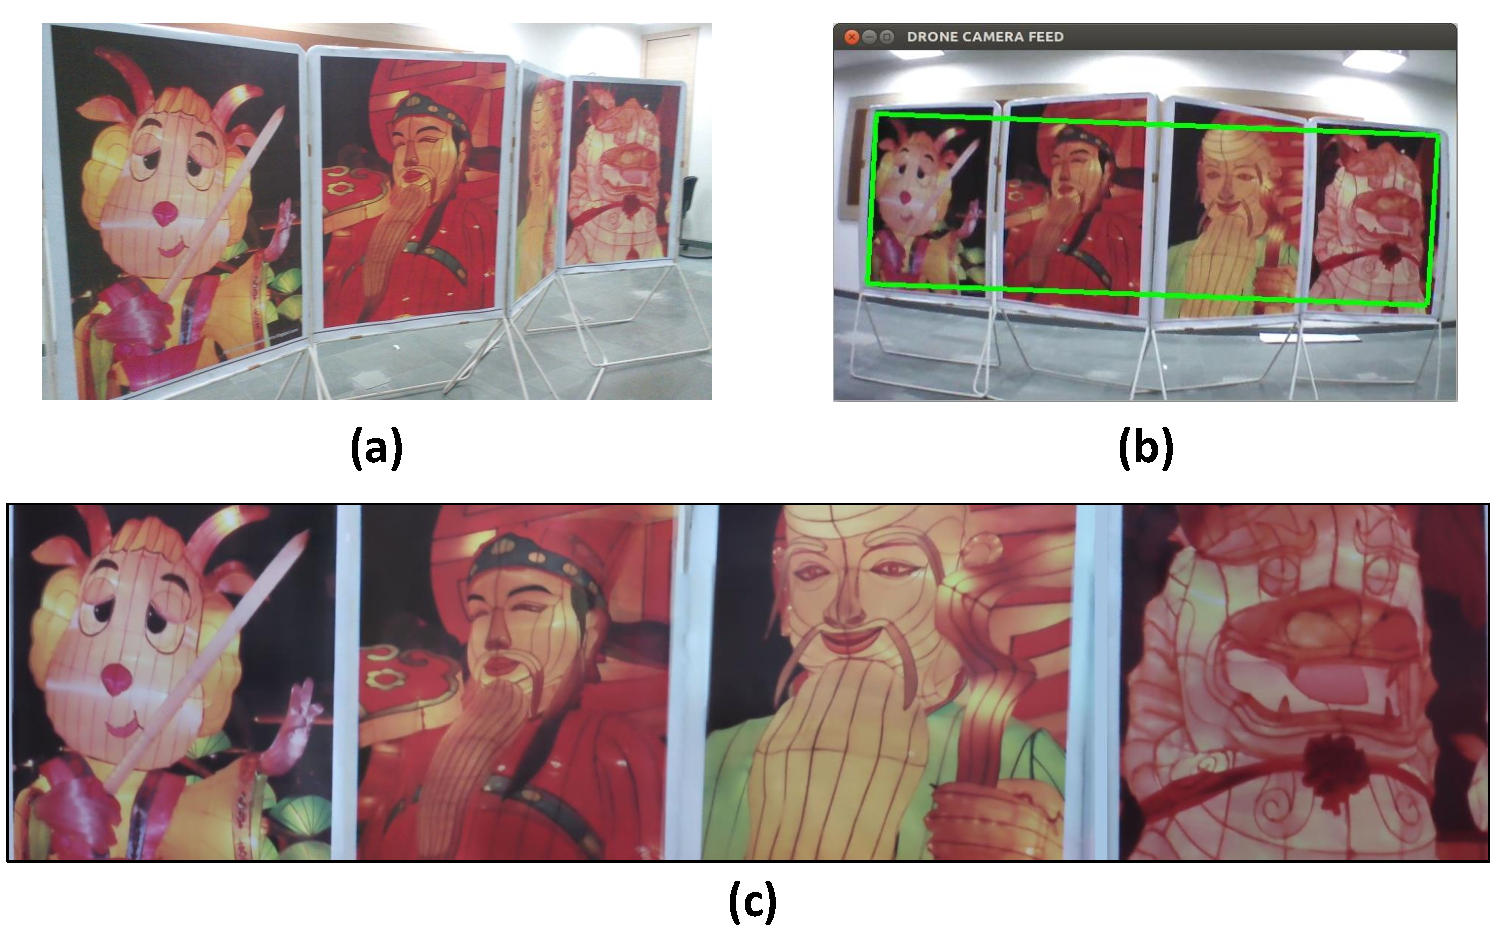
\includegraphics[width=0.98\linewidth]{figures/multiplanar/teaser2}
\caption[Overview of multiplanar imaging]{The multiplanar scene to be mosaiced is shown in (a). The long-range
photograph doesn't provide sufficient details of all the objects in the scene. A
quadcopter is maneuvered to allow a user to select the area of interest as shown
in (b). The final mosaicing output from this paper is shown in (c). The size of
our output is 3427 x 863 pixels.}
\label{fig:teaser}
\end{figure} 

\begin{figure}[htb]
\centering
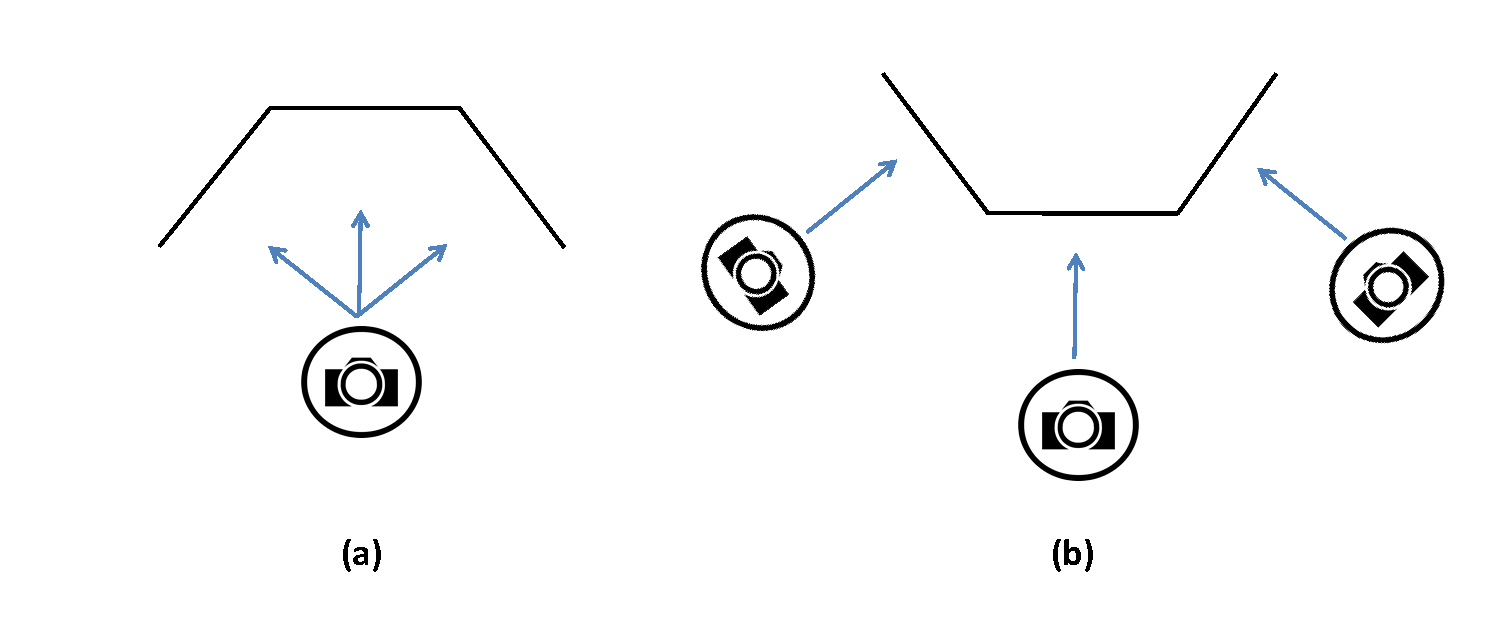
\includegraphics[width=\textwidth]{figures/multiplanar/ConcaveConvex}
\caption[Imaging concave surfaces versus convex surfaces ]{(a) Imaging concave surfaces. We do not
have to change our position, changing orientation is sufficient to capture the
whole surface. (b) While imaging a convex surface, one have to change the
position as well as the viewing angle. It makes the process
of building homography based panorama  theoretically impossible.}
\label{fig:convex_concave}
\end{figure}

However, in practice, when we use such cameras for capturing
panoramas, we do not get the close-up orthographic view of the scenes which are
present at a height or inaccessible to human. We also require a steady hand for
a long time while capturing panoramas which might be too tiring.

The limitation of cameras is that it can create a panorama with an orthographic
view, if the surface to be imaged is present on a single plane. We can also get
a panorama with an orthographic view, if the surface is concave and the camera
is kept at the center of the surface, as shown in 
Figure~\ref{fig:convex_concave}(a). However, if the surface (or part of it) is
convex,  as shown in Figure \ref{fig:convex_concave}(b), viewpoint (along with
the orientation) has to be changed while imaging. It prohibits the use of
panorama mode of most cameras. If any camera allows such panorama creation, the
output is distorted due to change in homography.

In scenarios where handheld devices cannot capture an orthographic view of a
large input scene, an inexpensive flying device such as a quadcopter can be
used. A quadcopter can cover any large scene with an orthographic view with
fine details (e.g., facial features of a person in Figure \ref{fig:teaser})
by flying in front of each part of the scene. However, manually controlling a
quadcopter to image a large multiplanar scene is a tedious task and hence
requires automation.

\textbf{Problem Definition}
Prasad et al.~\cite{Prasad16} have developed an imaging application with the use
of a quadcopter. It handles large scenes and scenes with featureless (vacant)
spaces.
%But a few things were not considered in \cite{Prasad16}.%
%The first one is regarding navigation and control of quadcopter.%
In \cite{Prasad16}, we have to manually navigate the quadcopter smoothly to
image large scenes from a close distance. There are various options available for manual
navigation and control of quadcopter. FPV (First Person View) controllers are
often used for controlling quadcopters. However, we have to do a lot of manual
adjustments while using FPV. Hence, if we have to capture large surfaces from a
specific depth, it would be very tiring. Also, it is not ensured that the
surface is imaged orthographically. There is a high probability of collision
between quadcopter and the imaging surface during these adjustments. 

Also in \cite{Prasad16}, the mosaicing algorithm could mosaic only if the scene
lies on a single planar surface. However, the real world is made-up of
multiplanar as well as curved surfaces. In fact, we have many circumstances where the input
scene is spread over multiple planes. In such cases, we would like to image each
planar region orthographically and then \textit{unroll} the whole scene by
joining the individual mosaics so that we get the output mosaic of the input scene as if it
is present on a single plane.
 
\textbf{Challenges}
We would like to autonomously navigate quadcopter to capture the whole scene.
Generally Global Positioning System (GPS) is used for navigation of UAVs. However, GPS
does not work effectively and precisely in indoor scenarios. Even in outdoor
scenario, we may not rely fully on GPS due to GPS jammer, spurious
signal, etc.. Hence, we require a reliable navigation system to maneuver the
quadcopter in an unknown environment.

A quadcopter has onboard an IMU (Inertial Measurement Unit)  which consists of
accelerometers, gyroscopes, and magnetometers. The IMU provides pose which can be
used to determine desired locations from where the whole scene can be covered.
Due to the jerky nature of an inexpensive quadcopter, the IMU sometimes
provide erroneous measurements  which result in incorrect pose information.
Thus, there is a requirement for further calibration. We require a way to
provide the quadcopter its precise pose in order to do the real-time calibration. A
technique named Parallel Tracking and Mapping(PTAM) is introduced
in~\cite{klein} to estimate camera pose in an unknown scenario. Engel et
al.~\cite{engel} have used both PTAM and IMU data to estimate correct
positional information.

A quadcopter can image the given area of interest provided by the user reliably
using pose estimates given by the method in \cite{engel}. However, even a
three-minute video captured by quadcopter, resulting in thousands of images
overwhelm any mosaicing application. Hence, instead of videographing the whole
area, the quadcopter should hover at certain points to take a stable video.
Later, appropriate images from all videos can be selected such that the whole
scene is covered in those images. We require an algorithm which calculates
those specific positions  where the quadcopter should hover and record an HD
video.

In the case of multiplanar surfaces, these problems worsen. For concave
surfaces (Figure \ref{fig:convex_concave}(a)), if the camera is placed at the
center of concave surface, imaging can be done from the single viewpoint.
However, if the plane is convex(Figure \ref{fig:convex_concave}(b)), viewpoints
as well as the orientation have to be changed. A quadcopter has to recognize
multiple planes in real-time and then change its direction for every plane before imaging the
region so that it becomes normal to the plane.

Though \cite{engel} gives accurate positional information, the roll and
pitch information is not reliable due to jerky motion of a quadcopter.
Additionally, 3D map output by \cite{engel} is an approximate sparse map of the
environment where some 3D points from the map may not be present in the real
scene. Hence, we cannot use only the 3D map to reconstruct the 3D world of input
scene. We may use homography based stitching for mosaicing individual planar
regions as it is more stable than 3D map building. Next, we can use plane
information and camera positions to join those mosaics to get an unrolled view
of the input scene.

\textbf{Contributions}
Our goal is to image multiplanar regions autonomously using a quadcopter. Initially,
3D positions of feature points on the imaging surface are estimated using a PTAM
based method. These positions are used to detect multiple planes in real-time
using J-linkage. Then, we ask the user to select the desired area spread over
multiple planes. Subsequently, positions of quadcopter for covering the user specified
area are calculated. These positions are such that user specified area is
covered with minimum images. 

Next, we fly the quadcopter orthographically to each plane and maneuver on
the planned path comprised of the estimated positions (calculated in the earlier
step). The quadcopter is hovered at each position for a small duration to capture the
video of a part of the whole scene. Images from each plane are individually stitched together
using feature based homography, i.e., we get individual mosaics per plane. Finally, we join
individual mosaics using positional information from the quadcopter to create the full mosaic.

The use of moving quadcopter for covering multiplanar surface may intrigue use
of Structure from Motion (SfM) paradigm. However, SfM provides a sparse 3D map
if there are insufficient number of feature points (as well as correspondences).
Also, if we do texture mapping on the sparse 3D map, the output is not satisfactory.
Instead, we use homography based stitching to mosaic individual planes and merge
them to get unrolled view which is more effective than using the sparse 3D map.


%Another minor problem with earlier method was: the quality of images. We were
%using images streamed over Wi-Fi channel which are of lesser size ($640 \times
%360$) than the size of images quadcopter stores on USB drive onboard i.e.,
%$1280 \times 720$. So, the quality of output mosaic would also be lesser. If we
%could synchronize the images stored on USB drive with the images streamed over
%Wi-Fi channel we could possibly get higher quality mosaic.

%The goal of this paper is to develop a method for autonomous control and
%navigation of quadcopter to cover the scene on a multiplanar surface. We also
%aim to provide unrolled view of a scene spread over multiplanar surfaces.

\section{Methodology}
The method adopted is pictorially depicted in the overview shown in Figure
\ref{fig:workflow} and is described in detail later on. In brief, we probe the
input scene through a quadcopter, calculate the 3D positions of feature points,
and detect bounded multiplanar regions from the area marked by the user through
our user interface. Path planning is done for each bounded planar region to find
out the camera positions. The quadcopter is autonomously maneuvered along the
estimated path and videos are captured at target points. For each bounded
planar region, the appropriate frame from each video is found and then supplied
to a mosaicing algorithm.  Finally, all mosaics are joined using the pose information from a quadcopter to get a full unrolled view.

\begin{figure}[ht!]
\centering
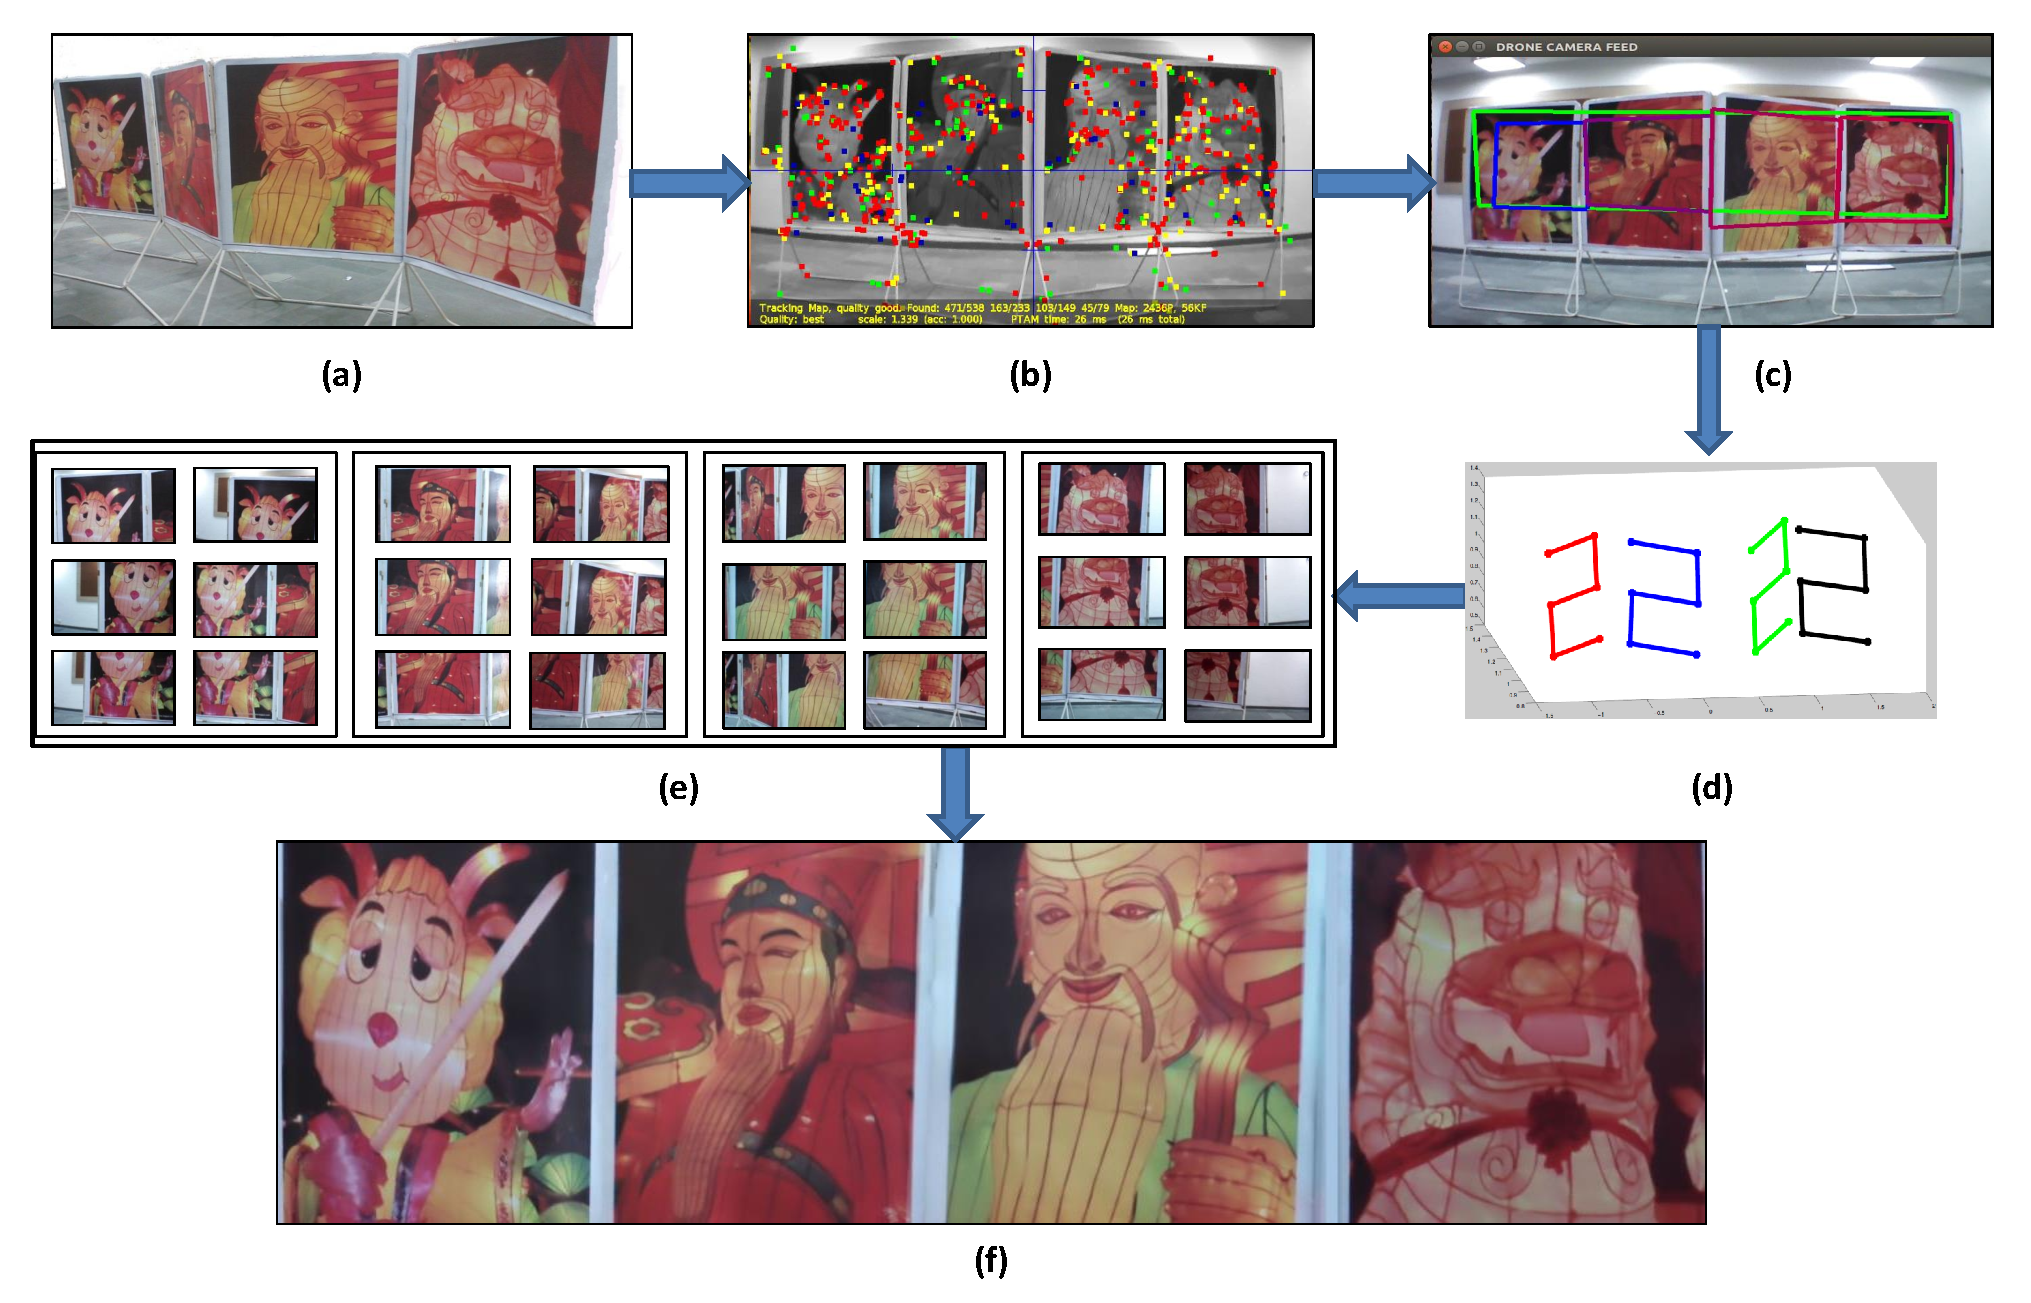
\includegraphics[width=\textwidth]{figures/multiplanar/workflow}
\caption[Overall Workflow]{Overview: (a) Input Scene to be imaged. (b) Feature points in the scene
are found, and their 3D positions are estimated using scale aware PTAM \cite{engel}. (c) Multiple bounded planar
regions are estimated using our algorithm. (d) For each bounded planar region, 3D camera positions
are calculated and overall path planning is done. (e) Videos are captured at
each target position. From each captured video, the appropriate frame is
found. (f) Individual mosaics are joined to get final output.}
\label{fig:workflow}
\end{figure}
\subsection{3D map}
We have used PTAM based method \cite{engel} to localize the quadcopter as well
as to create a 3D map of the surrounding environment (See Figure \ref{fig:ptam_output}).
In PTAM, initially, the prior pose is estimated using motion model. Then, the
map points are projected into the image using prior pose estimate. Next, the camera
pose is updated using some of the feature matches in the image. The final pose
estimate is computed from all the matches found.
 
The initial map built from stereo initialization algorithm has an arbitrary
scale. Hence, there is a requirement of scaling the  map to metric units. This
is done by assuming that the camera is translated 10 cm between the stereo pair. This
assumption may not be true in the case of an inexpensive quadcopter due to its jerky
motions. Hence, proper scale estimation is necessary.

\textbf{Scale Estimation}
A quadcopter measures a distance traveled during translation using PTAM as well
as available metric sensors (ultrasound altimeter) at regular intervals. We get
a pair of samples $\mathbf{x}_i, \mathbf{y}_i \in {\Re}^d$ where $\mathbf{x}_i$ is
scaled translation calculated from the PTAM system and $\mathbf{y}_i$ is the
distance measured by the metric sensor at each interval. These pair of samples are related
according to $\mathbf{x}_i \approx \lambda \mathbf{y}_i$. The scale $\lambda$ is
estimated by minimizing the negative log-likelihood\cite{engel}.  

We could get the correct pose by  scaling  PTAM estimated pose. However, we
cannot rely only on PTAM for pose estimation as visual feedback may lag due to
problems in wi-fi connectivity. Hence, there is a requirement of  alternative
mechanism as a fallback to PTAM. Engel et al. \cite{engel} have used Extended
Kalman Filter to fuse the odometry observation model with the visual observation
model for state prediction, i.e., estimating the pose (x,y,z and roll-pitch-yaw) of 
the quadcopter at any given instant.

\textbf{State Prediction and Observation:} The state space consists of a total
of ten state variables. 
\begin{ceqn}
\begin{align}
	\mathbf{x}_t &\coloneqq {(x_t, y_t, z_t, \dot{x_t}, \dot{y_t},
	\dot{z_t}, {\Phi}_t, {\Theta}_t, {\Psi}_t, \dot{{\Psi}_t} )}^T  \in
	{\mathbb{R}}^{10},
\end{align}
\end{ceqn}
where $(x_t, y_t, z_t)$ represents the position of the quadcopter in
metric units and $(\dot{x_t}, \dot{y_t}, \dot{z_t})$, the velocity in m/s, both
in world coordinates. The state also contains three angles (in degrees), i.e.,
the roll ${\Phi}_t$, pitch ${\Theta}_t$, and yaw ${\Psi}_t$, of the drone. 
An observation function $h(x_t)$ for each sensor as well as respective observation vector $z_t$
composed from the sensor readings is defined for each observation model.

\textbf{Odometry observation model:} A quadcopter measures its horizontal speed
(i.e., along x and y direction) in its local coordinate system which is
transformed into the global coordinate system to get $\dot{x_t}$ and
$\dot{y_t}$. The roll and pitch angles are directly taken from the
accelerometers' observations. Height measurements ($\hat{h_t}$) and yaw measurements
($\hat{{\Psi}_t}$) are differentiated and treated as observations of respective
velocities. The resulting observation function $h_I(\mathbf{x}_t)$ and
measurement vector $\mathbf{z}_{I,t}$ is given by,
\begin{ceqn}

\begin{align}
	h_I(\mathbf{x}_t) &\coloneqq  
	\begin{pmatrix} 
		\dot{x_t}\cos{{\Psi}_t} - \dot{y_t}\sin{{\Psi}_t} \\
		\dot{x_t}\sin{{\Psi}_t} + \dot{y_t}\cos{{\Psi}_t} \\
		\dot{z_t} \\
		{\Phi}_t \\
		{\Theta}_t \\
		\dot{{\Phi}_t}   	
	\end{pmatrix}
	\\
	\mathbf{z}_{I,t} &\coloneqq (\hat{v}_{x,t}, \hat{v}_{y,t}, (\hat{h}_t -
	\hat{h}_{t-1}), \hat{{\Phi}_t}, \hat{{\Theta}_t}, (\hat{{\Psi}_t} - \hat{{\Psi}}_{t-1}  ) )^T
\end{align}
\end{ceqn}
\textbf{Visual Observation Model:} The pose estimate is scaled by the
current estimate for the scaling factor ${\lambda}^{*}$ when PTAM tracks a
video frame successfully. This pose estimate is transformed from the coordinate
system of the front camera to the coordinate system of the quadcopter. Direct
observation of the quadcopter’s pose is given by,
\begin{ceqn}

\begin{align}
	  h_P(\mathbf{x}_t) &\coloneqq  {(x_t, y_t, z_t, {\Phi}_t, {\Theta}_t,
	  {\Psi}_t)}^T \\
	  \mathbf{z}_{I,t} &\coloneqq
	  f(\mathbf{E}_{\mathit{DC}}\mathbf{E}_{\mathit{C},t} )
\end{align}
\end{ceqn}

where $\mathbf{E}_{\mathit{C},t} \in SE(3)$ is the estimated camera pose (scaled
with $\lambda$ ), $\mathbf{E}_{\mathit{DC}} \in SE(3)$ the constant
transformation from the camera to the quadcopter coordinate system, and $f :
SE(3) \rightarrow \mathbb{R}^6$ the transformation from an element of $SE(3)$ to
our roll-pitch-yaw representation.

\textbf{Prediction Model:} The Extended Kalman filter is used to fuse all state
variables from both observation models. (Please see \cite{engel} for the
details). Finally, the prediction model describes how state vector $\mathbf{x}_t$
evolves from one timestep to next. The quadcopter’s horizontal acceleration $\ddot{x}, \ddot{y}$ is
approximated based on its current state $\mathbf{x}_t$.
The quadcopter's vertical acceleration   $\ddot{z}$, yaw-rotational 
acceleration $\ddot{{\Psi}_t}$ and roll and pitch rotational speeds,
$\dot{{\Psi}_t}, \dot{{\Theta}_t}$ are estimated based on the state
$\mathbf{x}_t$ and  active control command $\mathbf{u}_t$. Finally, using quadcopter's 
estimated pose information, we update the 3D map of the environment.

\noindent\textbf{Scale Accuracy:} 
Though \cite{engel}  gives a 3D map of the environment, the scale accuracy is
not ensured. It leads to inaccurate 3D coordinates of feature points. However, we
require accurate 3D coordinates of the region to be imaged for successful path
planning and its execution. To ensure accurate scale, we moved the quadcopter autonomously in
the vertical direction (up and down) by fixed distance. The reason behind moving in
the vertical direction is that the sonar gives us very accurate height information 
which is used to remove scale ambiguity.

We have conducted a small experiment to demonstrate the efficacy of our method to
achieve high scale accuracy. First, we initialized PTAM after
taking off the quadcopter, moved the quadcopter to location (0, 0, 1), i.e., 1
meter above the ground, and finally landed it at the same location. Ideally,
take-off location and land location should be same. However, due to errors in
PTAM initialization as well as noise in IMU measurements, the distance between
two locations will be non-zero. We use this distance as a measure of error. We
also tried to imbalance the quadcopter, while it is at location (0, 0, 1),
before landing to check its ability to come back to the original position.

Later, we repeated the experiment with one change, instead of using only PTAM
initialization, we have autonomously moved the quadcopter up and down by fixed
distance (1 meter) after PTAM initialization. Our summarized observations
after ten runs in both cases are listed in the Table~\ref{tab:ptamInit}.
\begin{table}
\centering
\newcolumntype{C}{ >{\centering\arraybackslash} m{2cm} }
\newcolumntype{D}{ >{\arraybackslash} m{5cm} }
\begin{tabular}{|D|C|C|C|C|}
\hline
\centering Case & Avg. Scale Accuracy & Avg. Scale (in m) & Number of Iterations &
Mean Error $\pm$ std. (in cm)\\
\hline
Only PTAM initialization & 0.524 & 1.2 & NA & 82.6 $\pm$ 10.73 \\
\hline
PTAM initialization with accuracy check & 1.0 & 2.33 & 3--4 & 13.2 $\pm3.6$\\
\hline       
\end{tabular}
\caption[Effect of ensuring scale accuracy on pose estimation]{Effect of
ensuring scale accuracy on the pose estimation of a quadcopter.
The first row shows that with only PTAM initialization, we do not get an accurate pose.
When we use our method to ensure high scale accuracy, we are much better in
pose estimation. The scene used for this testing was 2.3 meters away from the
quadcopter. As the estimated scale (2.33m) with our method is very close to the
actual distance of the scene from the quadcopter, the generated 3D map is also
very accurate.}
\label{tab:ptamInit}
\end{table}
Table~\ref{tab:ptamInit} clearly indicates that the pose estimate with only PTAM
initialization is far off (around 85cm) from the actual position\footnote{We also
noted that sometimes quadcopter was not able to come anywhere near to (0, 0, 1)
if we imbalance quadcopter purposefully after PTAM initialization.}.
However, when we ensure high scale accuracy, the estimated pose is within 15cm
of the actual location. The estimated scale is also very close to the actual distance of
the plane if we use our method for ensuring scale accuracy.

\begin{figure}[t!]
\centering
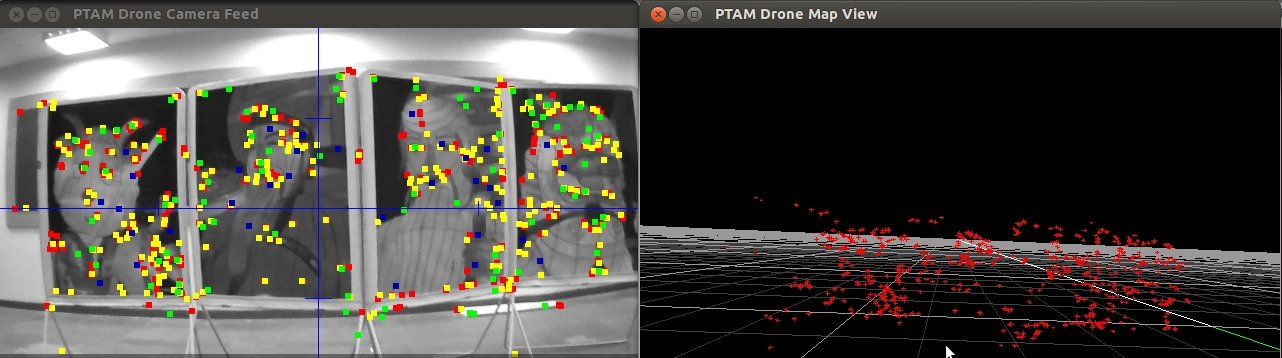
\includegraphics[width=\linewidth]{images/3D_2D}
\caption[Creation of 3D map]{Mapping of 3D locations to 2D image pixel locations
of feature points using PTAM. Left: Camera view showing 2D locations of detected feature points.
Color coding indicates the coarseness level of detected features. Right: Mapview
showing 3D locations of detected feature points.}
\label{fig:ptam_output}
\end{figure}

\subsection{Human Interaction}
Next step after we get a 3D map of the environment is getting the desired area for
imaging from the user. The user may be interested in a particular part of
the scene spread over multiple planes. Hence, we have to identify the user's
area of interest on the multiplanar surface. We first fly the quadcopter at a
sufficiently far distance from the surface. The distance should be such that the user can see the whole
scene. The user marks the area of interest with the provided user interface.\\
\begin{figure}[t!]
\centering
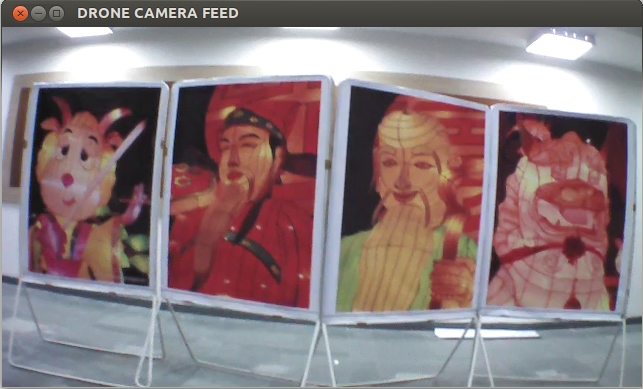
\includegraphics[width=0.31\linewidth]{images/UI_input}
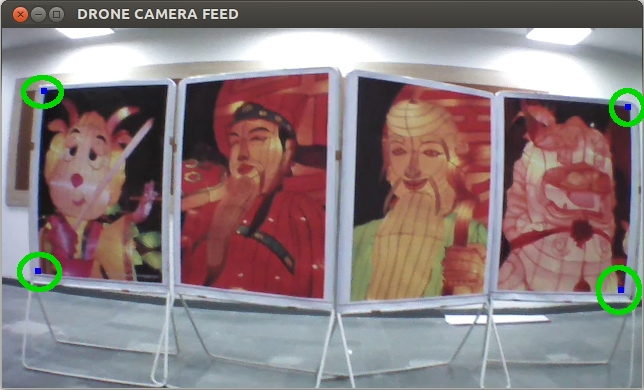
\includegraphics[width=0.31\linewidth]{images/UI_points_marked}
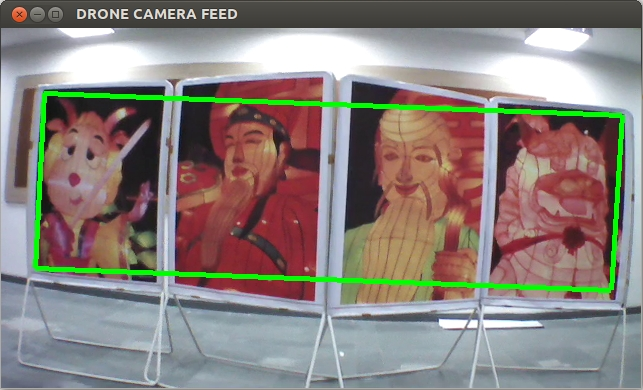
\includegraphics[width=0.31\linewidth]{images/UI_convexHull}
\caption[Our user interface]{Left: The user is shown a live video stream as seen
from a quadcopter camera. Middle: The user may click points to denote the area of interest. We 
find out the nearest 3D point and show its projection (encircled blue pixels) on
the image plane. Right: Once user finishes with clicking points, we find out its convex
hull and show it in green convex polygon.}
\label{fig:ui}
\end{figure}
\textbf{User interface} Users are shown the live video stream as seen through
the quadcopter (Figure \ref{fig:ui}(Left)). Now, users can click points to
mark their area of interest on the 2D screen. At the backend, we determine the
nearest 3D point corresponding to the location clicked by the user and then show
its projection on the image plane. (Figure \ref{fig:ui}(Middle)). Once they
finish marking the points, they can see the convex hull of the
clicked points to check whether the area to be covered is indeed the area of
interest (Figure \ref{fig:ui}(Right)). The user can optionally add or delete points
or even completely remove all clicked points using the interface and select the
new ones.

\subsection{Multiplanar Regions Detection}
We have to detect multiple planes present in the user's region of
interest. There are many algorithms such as Sequential RANSAC\cite{Kanazawa},
multiRANSAC\cite{zuliani} , J-linkage\cite{jlinkage}, T-linkage\cite{tlinkage}
etc. to detect multiple models from the data. We have chosen a real-time
implementation of J-linkage \cite{realtimejlinkage}.\\
\textbf{J-linkage:} Sequential RANSAC and multiRANSAC algorithms require
the number of planes as an input parameter. However, as the number of planes
change according to the input scene, we cannot use these algorithms. J-linkage and T-linkage
doesn't require the number of planes as an input parameter. 
%Though T-Linkage is more robust to noise in the input points, it is an order of
%magnitude slower than J-linkage. 
Our application requires real-time detection of the number of planes before proceeding for 
actual capture. This makes J-linkage more suitable than T-linkage.

However, J-linkage doesn't give the extent of the plane, i.e., the bounded
region. It tries to fit all points to the planes. Figure \ref{fig:multiplane}
depicts the relevant scenario. As we can see, there are some points which may
be the result of an inaccurate 3D map generated by PTAM (indicated by the black oval).
As these points have ``geometric'' affinity towards the plane A, J-linkage puts
these points in the plane A\textquotesingle s cluster. However, in the real world they
are part of the plane B. Hence, we have to disambiguate such points for
the correct calculation of bounded multiplanar regions. We have developed an
algorithm to modify the output of J-linkage to give correct bounded multiplanar regions.\\
\textbf{Improvement over J-linkage:} J-linkage algorithm outputs label
for each data point denoting to which plane that data point belongs. Our
algorithm does the following to find continuous bounded multiplanar regions
from J-linkage output:
\begin{itemize}
  \item Run clustering algorithm, e.g., k-means using the output of J-linkage
  as initial labels.
  \item Find out the distance of all points inside each cluster from the cluster
  centroid along the normal of the given plane.
  \item Remove the points from the cluster which are more than 95 percentile
  farther from the cluster centroid along the plane normal.
  \item Find out the bounding rectangle of each cluster.
  \item Extend the rectangle till the intersection with the successive plane.
\end{itemize}

This process is illustrated in Figure \ref{fig:multiplane}. J-linkage
gives us the labeling according to each point's vicinity to the detected
planes. However, the 3D points estimated by PTAM may be erroneous due to noise,
marked by circles in Figure \ref{fig:multiplane}(Top). J-linkage gives us wrong bounded
regions as these points do not belong to the planes labeled by it . Hence, we
run the k-means algorithm using the initial labels given by JLinkage. Now, points  
belong to the correct cluster as shown in Figure \ref{fig:multiplane}(Middle). 
However, we don't want points which are far away from the plane in the normal direction.
Hence, we remove those points which are more than 95 percentile farther from the cluster 
centroid along the plane normal. We also trim the boundaries of the plane by the bounding box of the
enclosed points. The final output is shown in the Figure \ref{fig:multiplane}(Bottom).

\begin{figure}[h!]
\centering
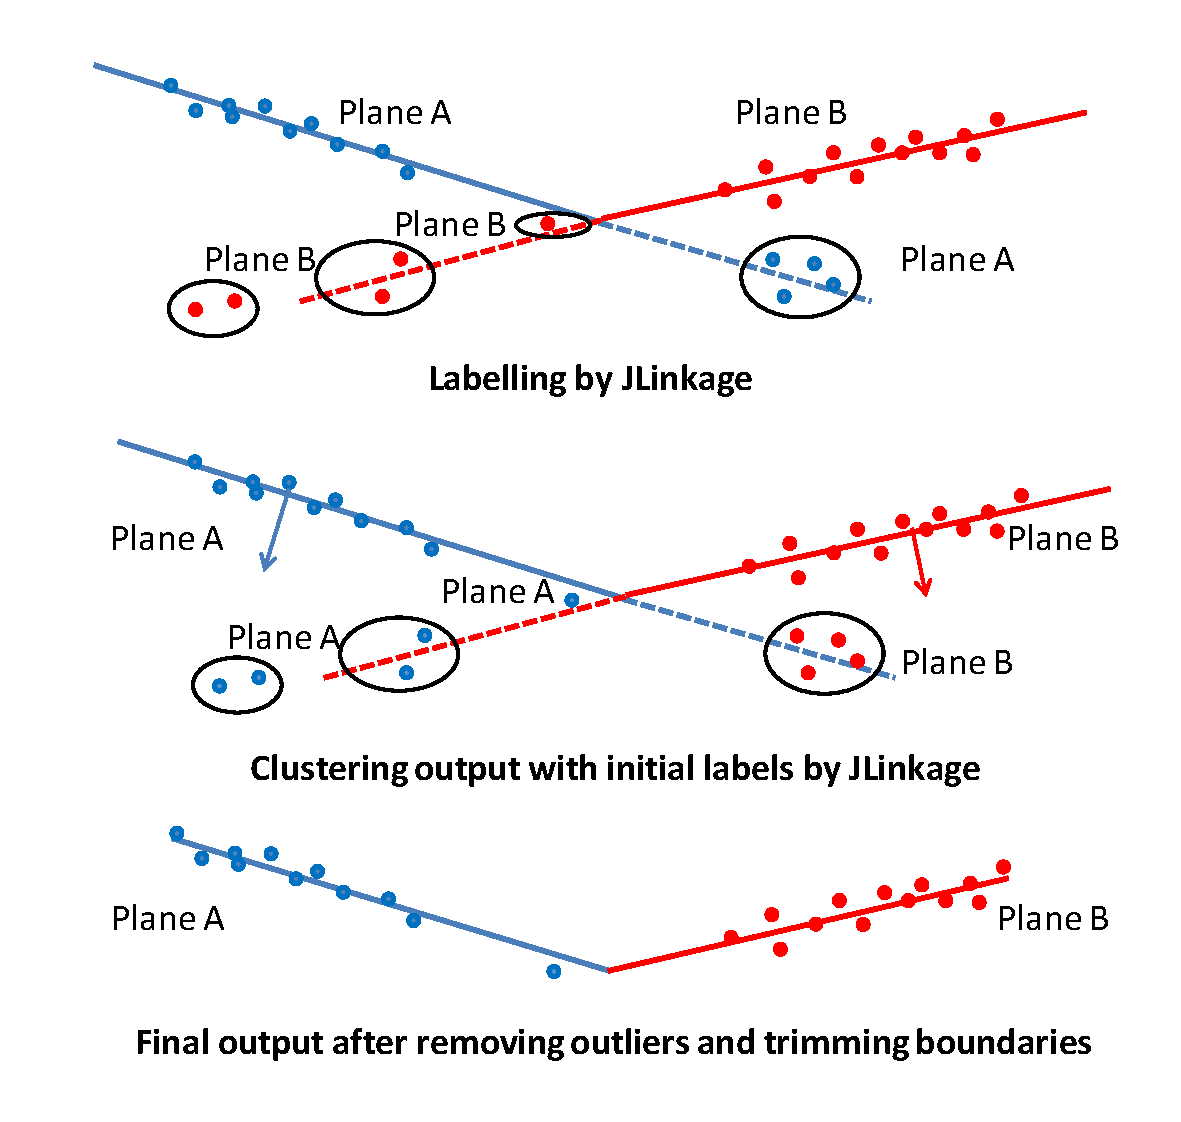
\includegraphics[width=\linewidth]{figures/multiplanar/multiplaneDetection}
\caption{Process of finding bounded multiplanar regions from J-linkage output.
The top image shows us the initial labeling given by J-linkage. Later, we run
the k-means algorithm using the initial labeling given by J-linkage. The output
is shown in the middle figure. Finally, we remove outliers which are farther from the
plane along normal direction and trim boundaries of the plane as shown in
the bottom figure.}
\label{fig:multiplane}
\end{figure}

Each bounded planar region is used to determine the path along which
the quadcopter is navigated to image that region.

\subsection{Path Planning}
The bounded region is divided into a grid of overlapping cells as shown in
Figure \ref{fig:grid}. We intend to cover each cell in a single image and then
use images from all cells to create a mosaic of a given bounded planar
region. The cell area (width, height) is decided on the basis of the amount of
details required of the scene. For example, if we have to probe our scene with
minute details, we have to go nearer to the plane. Hence, in that case, the
cell area is smaller. We require an overlap between neighboring images for
successful mosaicing. The amount of overlap between two cells is a function of
the required overlap in the feature space required for stitching. Currently,
the overlap is set at thirty percent of the cell area to deal even with sparser
(containing very fewer feature points) images.

\begin{figure}[h!]
\centering
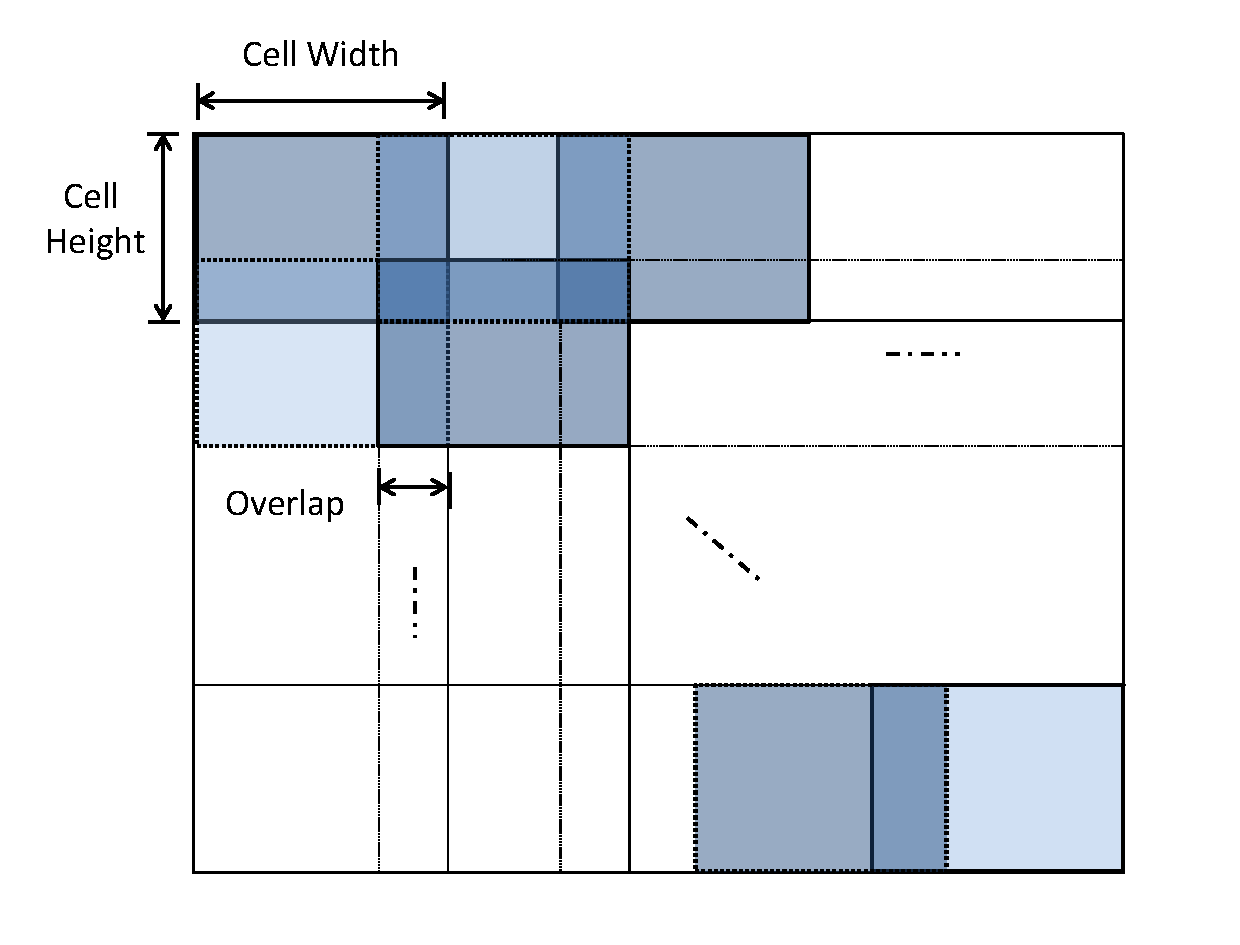
\includegraphics[width=\linewidth]{figures/multiplanar/PathPlanningGrid}
\caption{Grid of overlapping cells designed for path planning. We create a
grid for each bounded planar region. The cell width and the cell height is
decided based on the area we would like to capture in one frame. Overlap parameter is
a function of overlap required in feature space for successful stitching.
We find the camera position for each cell in the grid which in turn
gives us the path for a quadcopter to image the given bounded planar region.}
\label{fig:grid}
\end{figure}

Once we calculate coordinates of cell corners, we determine the desired position of
a camera from where the whole cell area is covered in a single image. It is
illustrated in the Figure~\ref{fig:solvepnp}. The coordinates of corner points
are decided on the basis of cell width, cell height and the top-left corner of
the cell. The image coordinates (in pixels) depends on the size of the image. We
pose this problem as a point correspondence problem to estimate the position
of the camera. We repeat this process for each cell to find out the waypoints of
the path of a quadcopter to cover the region in optimal (in a number of positions)
manner, so that the whole region is captured.

\begin{figure}[h!]
\centering
\includegraphics[width=\linewidth]{figures/multiplanar/solvepnp}
\caption{Finding the camera position for capturing the desired cell area in a
single image. Note that, imaging area coordinates are in metric units, while image
coordinates are in pixels. We use point correspondence problem to estimate the
camera position.}
\label{fig:solvepnp}
\end{figure}

\subsection{Navigation of a quadcopter}
 We use the pose estimate provided by PTAM  based method \cite{engel}to track
 the quadcopter during navigation along the planned path.\\
\textbf{Covering a bounded single planar region}:
We navigate the quadcopter smoothly in a ``snake scan'' manner along the target points estimated in path
planning step to cover each bounded planar region.\\
\textbf{Transition from one plane to another plane}: We make sure the
transition in terms of yaw as well as horizontal movement is smooth. To achieve this,
we divide the horizontal distance into three parts and  move along x-axis and y-axis
alternatively. During each step, we change the yaw in equal proportion so that
the quadcopter’s view is not changed drastically, which is very important for
tracking using PTAM \cite{engel}.

\subsection{Recording video and ROS streams}
%AR Drone doesn't have the capability of taking still photographs. 
 We are not sure about the exact position of a quadcopter while capturing
 images due to the error in PTAM as well as the jerky motion of a quadcopter. 
 Hence, instead, we record a video on the USB device onboard a quadcopter for a
 small amount of time (3 seconds) when we are in proximity of each point in the calculated path. We
also record ROS streams (image as well as positional data) captured over Wi-Fi.

\noindent\textbf{Finding the sharp and exact image from video:} We have to find
the sharp image, i.e., an image with the minimum blur which is closest to the
target point from 3 seconds HD video (approximately 90 images) to create a
mosaic. However, there is no positional data available on USB device. Positional
data stream and image stream captured over Wi-Fi help us in this process. First, we synchronize these
two streams captured over Wi-Fi using timestamp information. It gives us an
approximate position of each image from the image stream captured over Wi-Fi.
Now, we select the sharpest image among the images captured over Wi-Fi which
are taken from the positions in a proximity of the specified point. Later,
we match each image from the HD video (recorded on USB device) with the
selected image (selected from the Wi-Fi image stream) using SURF features. It
gives us a subset of HD images which are within a threshold in SURF\cite{Bay} feature
space from the selected image. Finally, we select the sharpest image from that subset of HD images.

\subsection{Creating mosaic of the bounded multiplanar region}
Once images for each bounded planar region are extracted from captured
videos, mosaic for each planar region is created using the method of creation of
a mini-panorama presented in \cite{Prasad16}. In \cite{Prasad16}, first images
are arranged in a rectangular grid according to their positions. Here, as we
already have grid information (created in path planning step), our first step
is done. Later, we do feature matching among the neighborhood images and create
the maximum spanning tree using the homography inliers as weight.  Finally,
mosaic, i.e., mini-panorama is created by warping images according to the
respective homography matrix (w.r.t. the  reference image).

\begin{figure}[ht!]
\centering
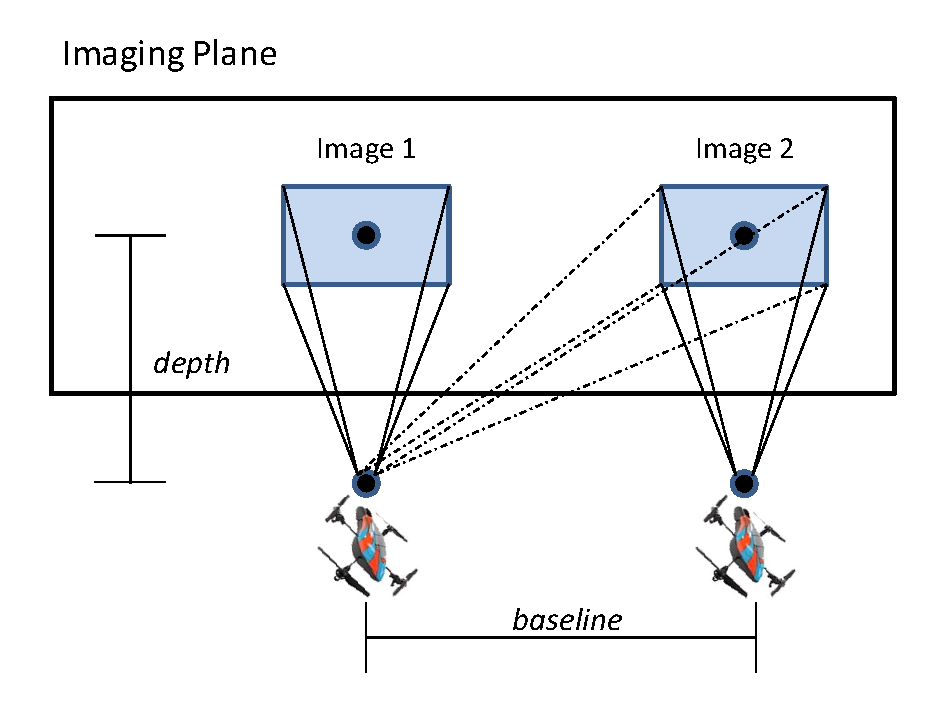
\includegraphics[width=\linewidth]{figures/multiplanar/SinglePlaneMosaic}
\caption{Super panorama creation by finding the disparity between reference
images of mosaics imaged on a single plane~\cite{Prasad16}.}
\label{fig:singlePlaneMosaic}
\end{figure}

After the creation of mini-panorama for each planar region, we join all
mini-panoramas using a method similar to the creation of super panorama used
in~\cite{Prasad16}. Super panorama is created by forming a simplistic stereo
pair between two images captured from the same depth, as shown in
Figure~\ref{fig:singlePlaneMosaic}. Using the stereo disparity formula, 
\begin{ceqn}
\begin{align}
\textit{disparity} = \textit{focal
length}\frac{\textit{baseline}}{\textit{depth}},
\label{eq:disparityOrig}
\end{align}
\end{ceqn}
we can ``place,'' from the first viewpoint, the image captured from the second
viewpoint, thereby creating a super-panorama. In~\cite{Prasad16}, the disparity
between the reference images of each mini-panorama is calculated by using the
distance between the camera and the imaging plane, i.e., the depth, and distance
between camera positions of reference images for each mini-panorama, i.e., the
baseline.

\begin{figure}[ht!]
\centering
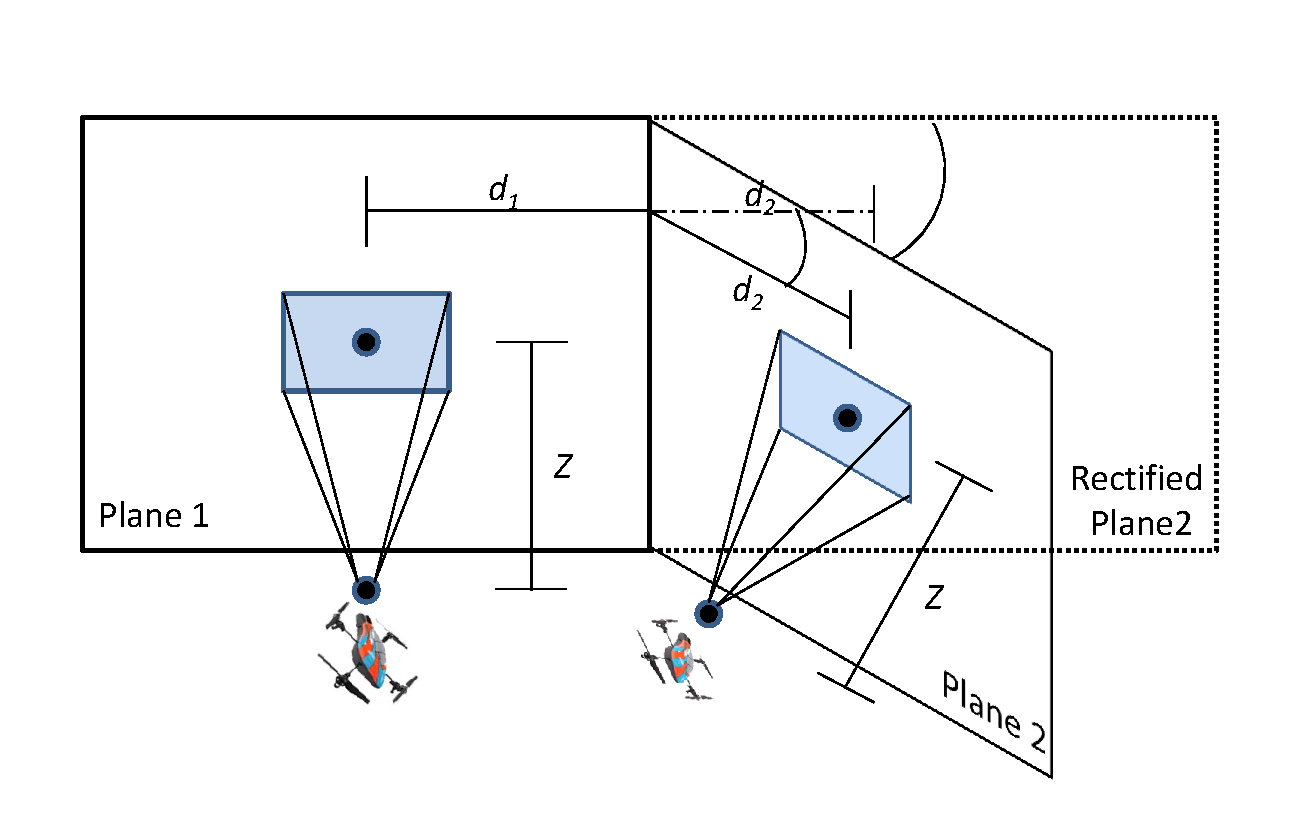
\includegraphics[width=\linewidth]{figures/multiplanar/MultiplanarMosaic}
\caption{Process of finding the disparity between reference images of mosaics
imaged on two different planes.}
\label{fig:multiplanarMosaic}
\end{figure}

In~\cite{Prasad16}, as all mini-panoramas were in the same plane, simple stereo
formulation (without rectification) was enough. In our case, as mini-panoramas belong to
multiple planes, we have to project mini-panoramas on any one plane to find the
disparity between reference images of all mini-panoramas. It requires image
rectification. However, as we keep the quadcopter's camera normal to the plane
while capturing images from each planar region, we don't have to do full
rectification. We just have to calculate the distance between the center of
projections, projected on the imaging plane, along the planes as shown in
Figure \ref{fig:multiplanarMosaic}.

Let us assume that the depth of the camera from both the imaging planes is same
(say $Z$). Now, the disparity of the image on the second plane with respect to
the image on the first plane is given as follows:
\begin{ceqn}
\begin{align}
\textit{disparity} = \textit{focal length}\frac{(d_1+d_2)}{Z},
\label{eq:disparity}
\end{align}
\end{ceqn}
where $d_1$ and $d_2$ are distances of projections of camera positions on the
first and second plane respectively, from the line of intersection of two
planes, and $Z$ is the depth of the camera from the plane.
If we compare Eq.~\ref{eq:disparityOrig} and Eq.~\ref{eq:disparity}, we can 
easily see that, now our baseline is $(d_1 + d_2)$, i.e., distance between
camera positions calculated along the plane, instead of calculating the direct 
distance between camera positions. The reason behind this difference is, imaging
areas are on two different planes instead of one.

If the center of projections are at different depths (e.g., say $Z_1$ and
$Z_2$), first we bring the image captured from lesser depth (say $Z_1$) to the
same depth of another image (which is captured from larger depth, say $Z_2$) by
zooming out by the fraction $\frac{Z_1}{Z_2}$. Later, we use Eq.
\ref{eq:disparity} to calculate the disparity by setting $Z=Z_2$.

To summarize, our method first creates an accurate 3D map of the input scene
spread over multiple planes using extended PTAM initialization. Next, we determine the
boundaries of each planar region using the improvised J-linkage algorithm.
Further, we estimate the optimal number of positions along which we will navigate the
quadcopter to capture videos which encompass the complete scene. Later, we
create the individual mosaics for each plane with the images extracted from
videos. Finally, the individual mosaics are joined using super-panorama
formulation to get an unrolled view of the input scene.

\section{Experiments and Results}
All our experiments have been completed with the inexpensive consumer
quadcopter called  Parrot’s AR Drone 2.0. The camera resolution of AR Drone 2.0
is 1280 $\times$ 720\footnote{But when we stream the image over Wi-Fi the resolution
of an image is 640 $\times$ 360.}. We have used ROS based ARDrone Autonomy
Driver~\cite{ardroneDriver} to communicate with the drone. We have also used
tum\_ardrone package~\cite{tumardrone} for ROS to do PTAM based state
estimation. We have developed an ROS node for autonomous navigation of
quadcopter. The code is developed in C++ and will be made available at
after acceptance of the paper. Mosaicing algorithm is also
developed in C++ using the OpenCV library (OpenCV 2.4.9). Experiments were
performed on a laptop with Intel Core i5 processor(@2.4GHz) and 8GB RAM.

We also took a picture of the scene, from a distance with a five mega-pixel
camera to better understand the scene as well as to show the efficacy of
our method.

\subsection{Single Plane with Multiple Visits}
We have first used our algorithm to image a single planar wall shown in
Figure \ref{fig:resultLady}(Left). As the wall was too tall and it was not
possible to view the full wall in one flash due to a shortage of space, we
selected the desired area in two steps as shown in Figure  \ref{fig:resultLady}(Middle). In path planning 37 (12
for the top part and 25 for the bottom part) positions were estimated to
encompass the user-selected area. Images captured from those positions are
mosaiced using our algorithm to get the final mosaicing output as shown in Figure \ref{fig:resultLady}(Right).
\begin{figure}
\centering
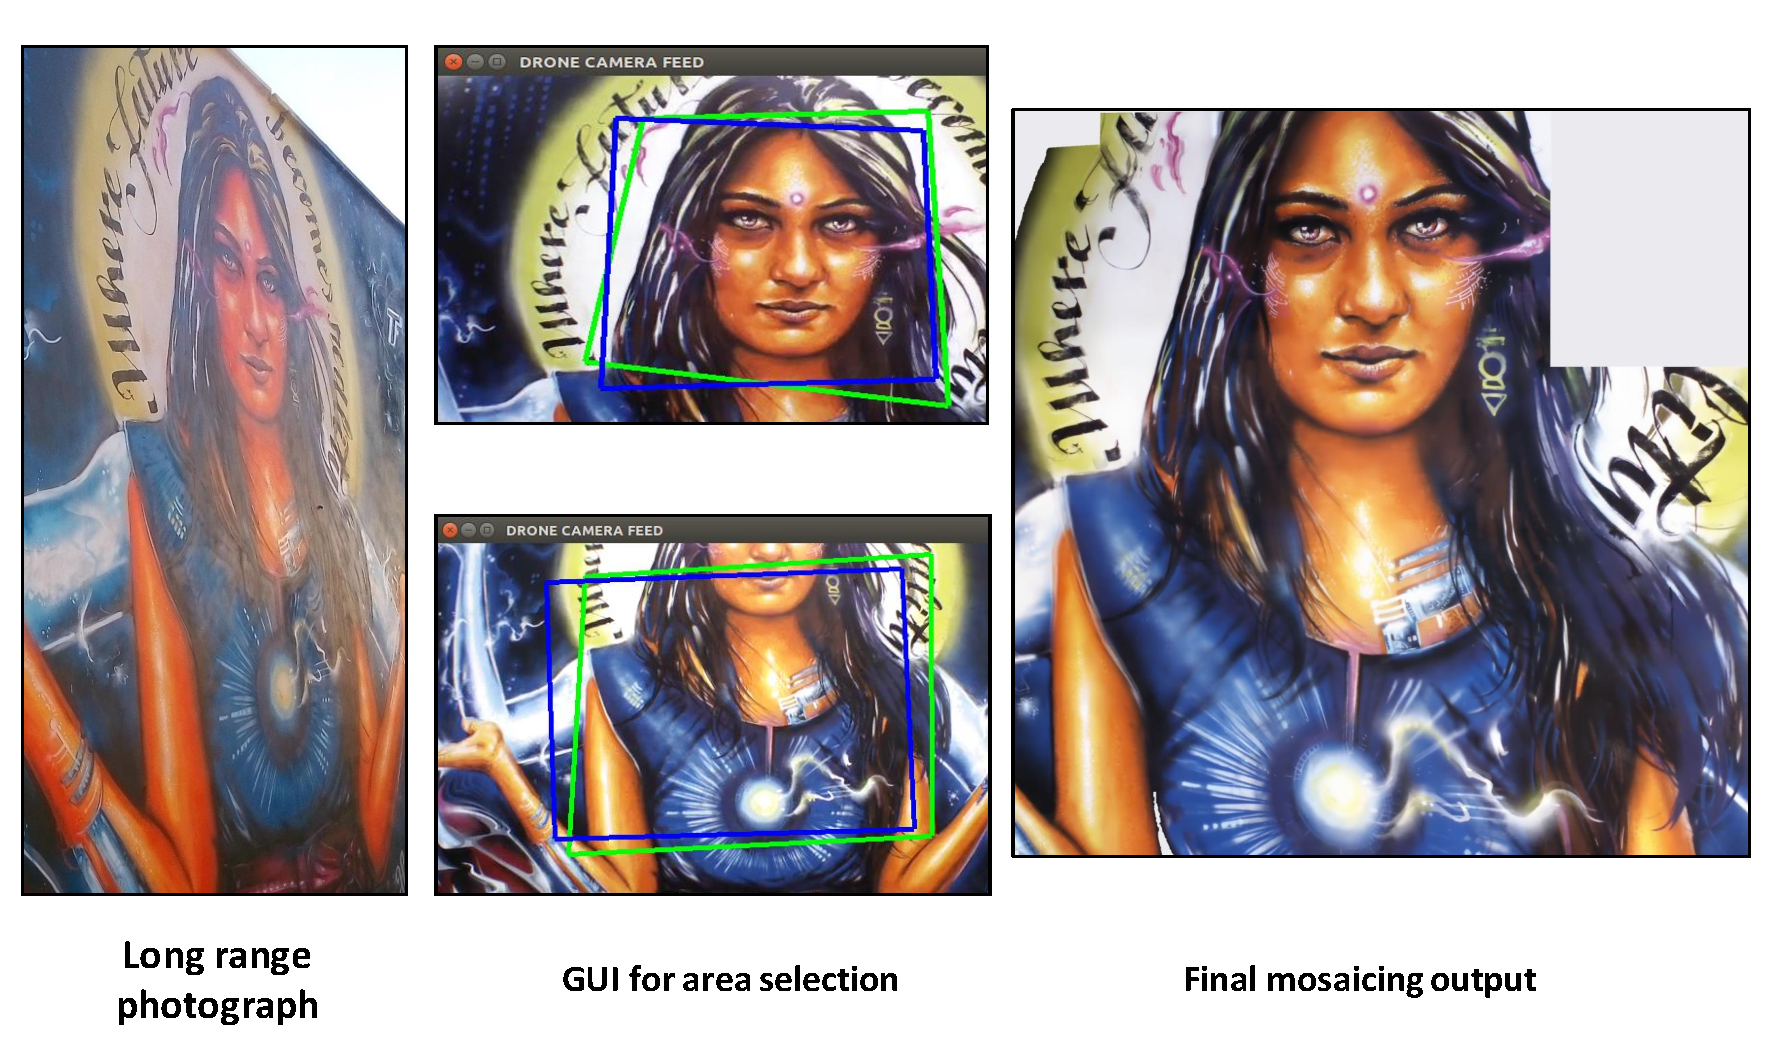
\includegraphics[width=0.9\textwidth]{figures/multiplanar/ladyResult.pdf}
\caption{There is a 15 feet tall wall as shown in the long-range photograph
(left) which we would like to image orthographically with details. We cannot
select the whole area in a single instance as we cannot go back to see the whole
wall. Hence, we selected the desired area in two steps as shown in GUI for area
selection (middle-top and middle-bottom). Green quadrilateral shows user selected area
while blue quadrilateral shows the bounded planar region estimated by our
algorithm. In path planning 37 (12 for the top part and 25 for the bottom part) positions were
estimated to encompass the user-selected area. Images captured from those
positions are mosaiced using our algorithm to get the final mosaicing output as shown in the
right image.}
\label{fig:resultLady}
\end{figure}

\subsection{Multiple Planes}
Our further experiments are done on various setups covering multiple planes.\\

\textbf{Concave:} In this experiment, the exhibits were arranged in the concave
fashion as shown in Figure \ref{fig:resultConcave}(Top-Left). We have selected
the area to be imaged as shown in Figure \ref{fig:resultConcave}(Top-Right). In
the path planning stage, overall 27 (9 from the left plane, 12 from the middle
plane, and 6 from the right plane) positions were estimated to encompass
user-selected area. Images captured from those positions are mosaiced using our
algorithm to get the final mosaicing output as shown in the Figure \ref{fig:resultConcave}(Bottom).

\begin{figure}
\centering
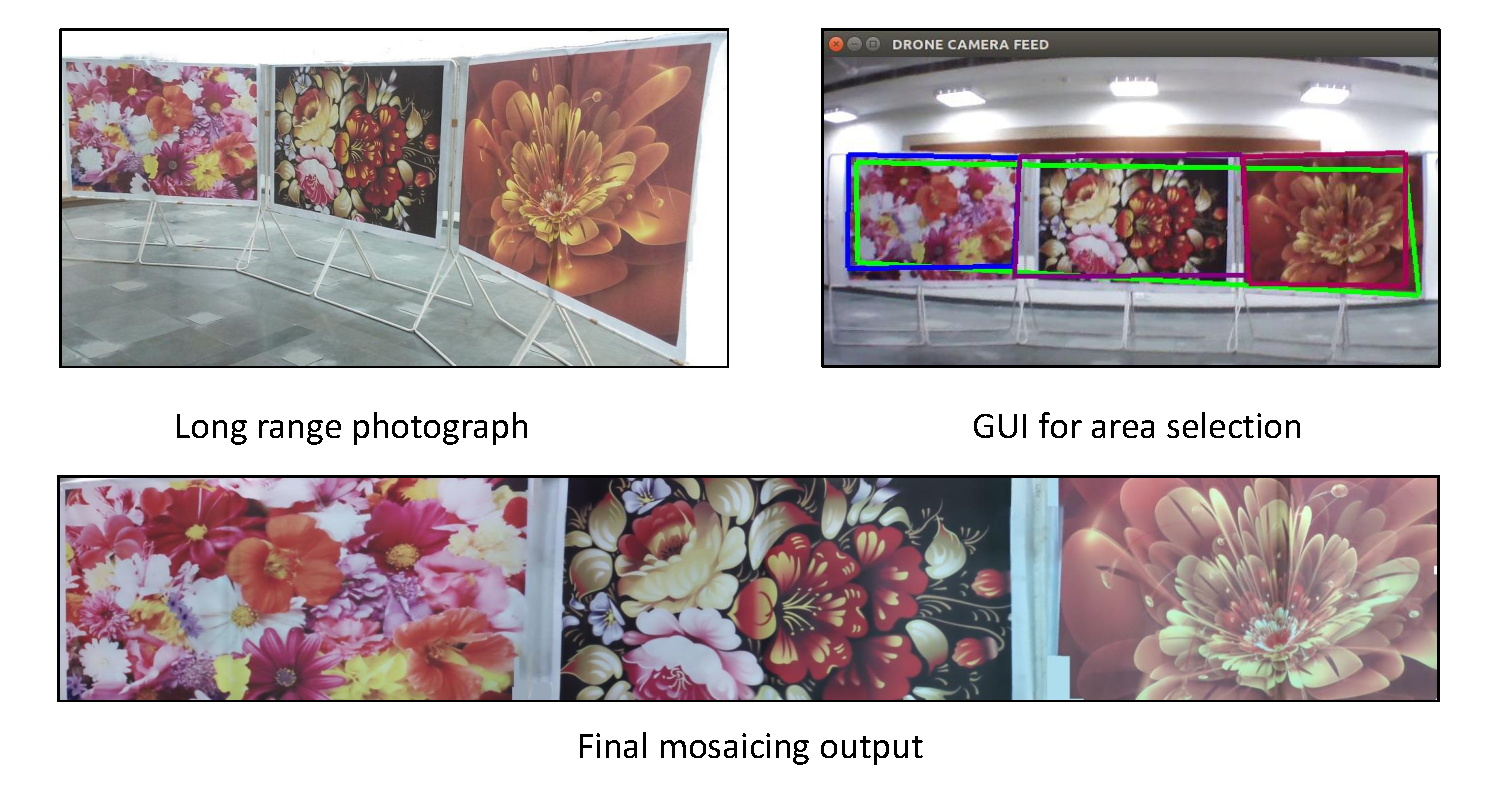
\includegraphics[width=\linewidth]{figures/multiplanar/ConcaveResult.pdf}
\caption[Result: Concave arrangement]{There is an art exhibition containing
multiple posters arranged in concave fashion as shown in the long range photograph (top-left). We have
selected the area to be imaged as shown in GUI for area selection(top-right).
Green quadrilateral shows user selected area while blue, violet and magenta
colored quadrilaterals represent the multiple bounded planar regions
estimated by our algorithm. In the path planning stage, overall 27 (9 from the left
plane, 12 from the middle plane, and 6 from the right plane) positions were
estimated to encompass the user-selected area. Images captured from those
positions are mosaiced using our algorithm to get the final mosaicing output as shown in the bottom image.}
\label{fig:resultConcave}.
\end{figure}

\textbf{Convex:} In this experiment, paintings were arranged in the convex
fashion as shown in Figure \ref{fig:resultConvex}(Top-Left). We have selected
the area to be imaged as shown in Figure \ref{fig:resultConvex}(Top-Right). In
the path planning stage, overall 30 (9 from the left plane, 12 from the middle
plane, and 9 from the right plane) positions to encompass user-selected area are
estimated. Images captured from those positions are mosaiced using our algorithm to get the final
mosaicing output as shown in the Figure \ref{fig:resultConvex}(Bottom).

\begin{figure}[t!]
\centering
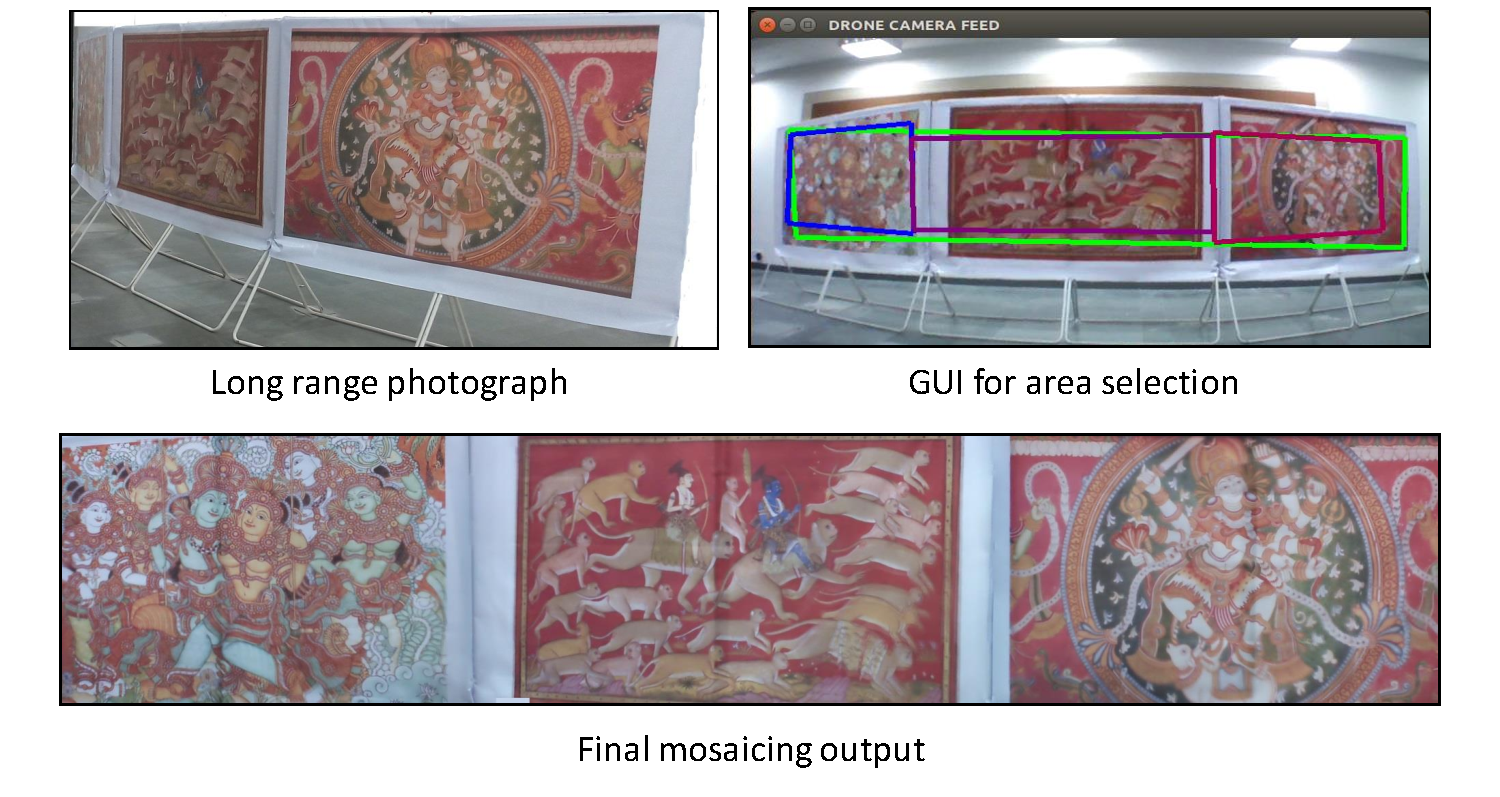
\includegraphics[width=\linewidth]{figures/multiplanar/convexResult.pdf}
\caption[Result: Convex arrangement]{There is an exhibition of Indian temple
paintings arranged in convex fashion as shown in the long range photograph (top-left). Note that we
cannot cover all paintings with enough details simultaneously. We have selected
the area to be imaged as shown in GUI for area selection (top-right).
Green quadrilateral shows user selected area while blue, violet and magenta
colored quadrilaterals represent the multiple bounded planar regions
estimated by our algorithm. In the path planning stage, overall 30 (9 from
the left plane, 12 from the middle plane, and 9 from the right plane) positions were
estimated to encompass the user-selected area. Images captured from estimated
positions are mosaiced using our algorithm to get the final mosaicing output as shown in
the bottom image.}
\label{fig:resultConvex}
\end{figure}

\textbf{Mixed:} We have performed a couple of experiments where the posters were
arranged in mixed fashion. The first arrangement looked like Figure
\ref{fig:resultMixed1}(Top-Left) where the middle posters form the convex region
while the side posters form the concave region. The selected area for imaging is
shown in Figure \ref{fig:resultMixed1}(Top-Right). In path planning overall 24 (6 from each
plane) positions are estimated to encompass the user-selected area. Images
captured from those positions are mosaiced using our algorithm to get the final mosaicing
output as shown in the \ref{fig:resultMixed1}(Bottom).

\begin{figure}[t!]
\centering
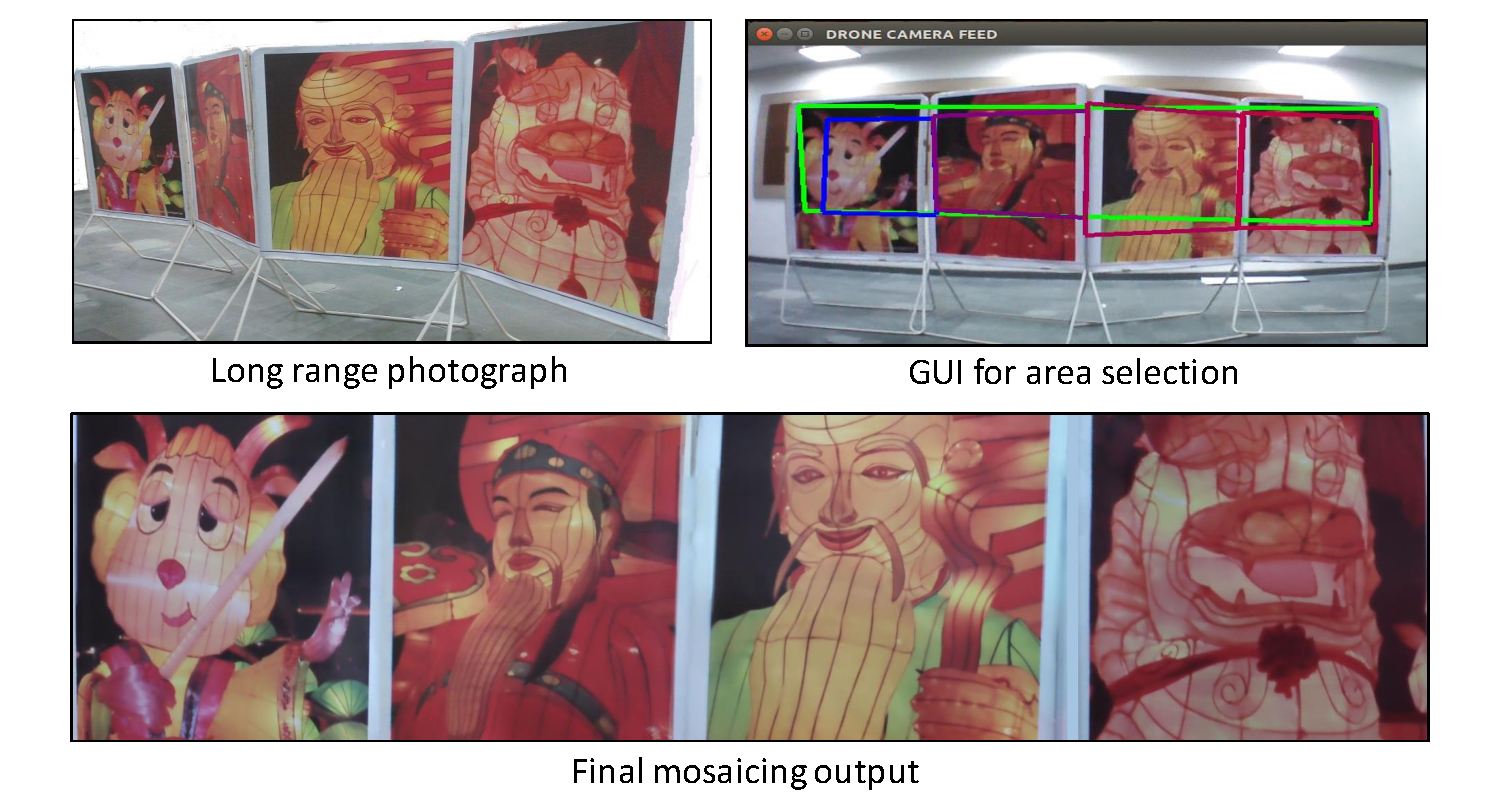
\includegraphics[width=\linewidth]{figures/multiplanar/mixed1Result.pdf}
\caption[Result: Mixed arrangement]{There is an exhibition of Chinese lanterns'
posters arranged in mixed (concave and convex) fashion as shown in the long range photograph
(top-left). Note that we cannot cover all paintings with enough details
simultaneously. We have selected the area to be imaged as shown in GUI for
area selection (top-right). Green quadrilateral shows user selected area while
blue, violet and magenta colored quadrilaterals represent the multiple
bounded planar regions estimated by our algorithm. In the path planning overall
24 (6 from each plane) positions were estimated to encompass the user-selected
area. Images captured from estimated positions are mosaiced using our algorithm to get the
final mosaicing output as shown in the bottom image.}
\label{fig:resultMixed1}
\end{figure}

In the second mixed arrangement, middle posters form the concave region while
 side posters form the convex region as shown in Figure
\ref{fig:resultMixed2}(Top-Left). The selected area for imaging is shown in
Figure \ref{fig:resultMixed2}(Top-Right).  In path planning overall 24 (6 from
each plane) positions were estimated to encompass the user-selected area.
Images captured from estimated positions are mosaiced using our algorithm to get the final mosaicing
output as shown in the Figure \ref{fig:resultMixed2}(Bottom).

\begin{figure}
\centering
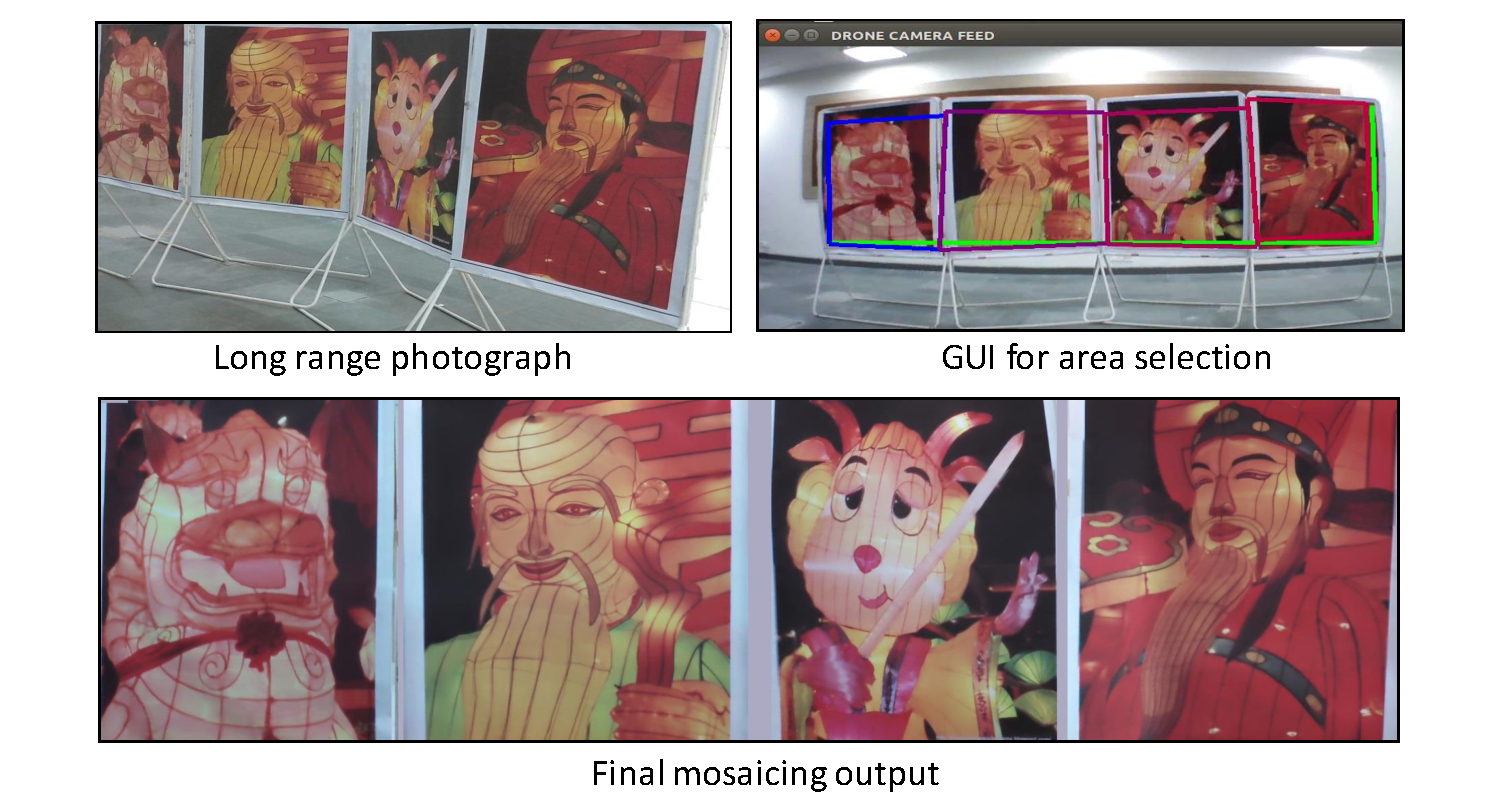
\includegraphics[width=\linewidth]{figures/multiplanar/mixed2Result.pdf}
\caption[Result: Mixed arrangement]{There is an exhibition of Chinese lanterns'
posters arranged in mixed (concave and convex) fashion as shown in the long range photograph
(top-left). Note that we cannot cover all paintings with enough details
simultaneously. We have selected the area to be imaged as shown in GUI for
area selection (top-right). Green quadrilateral shows user selected area while
blue, violet and magenta colored quadrilaterals represent the multiple
bounded planar regions estimated by our algorithm. In the path planning
stage, overall 24 (6 from each plane) positions were estimated to encompass the
user-selected area. Images captured from estimated positions are mosaiced using
our algorithm to get the final mosaicing output as shown in the bottom image.}
\label{fig:resultMixed2}
\end{figure}

\textbf{Planes at different depth:} In this experiment we have arranged posters
parallel to each other, but at different depths, as shown in Figure
\ref{fig:resultFrontBack}(Top-Left). It is not possible to mosaic them together
due to change in planes. However, we have imaged each exhibit independently
using quadcopter and brought the mosaic of the exhibit at a larger depth to the same depth
of lesser depth exhibit mosaic using the estimated plane equations' information.
The final result is shown in the Figure \ref{fig:resultFrontBack}(Bottom).
\begin{figure}
\centering
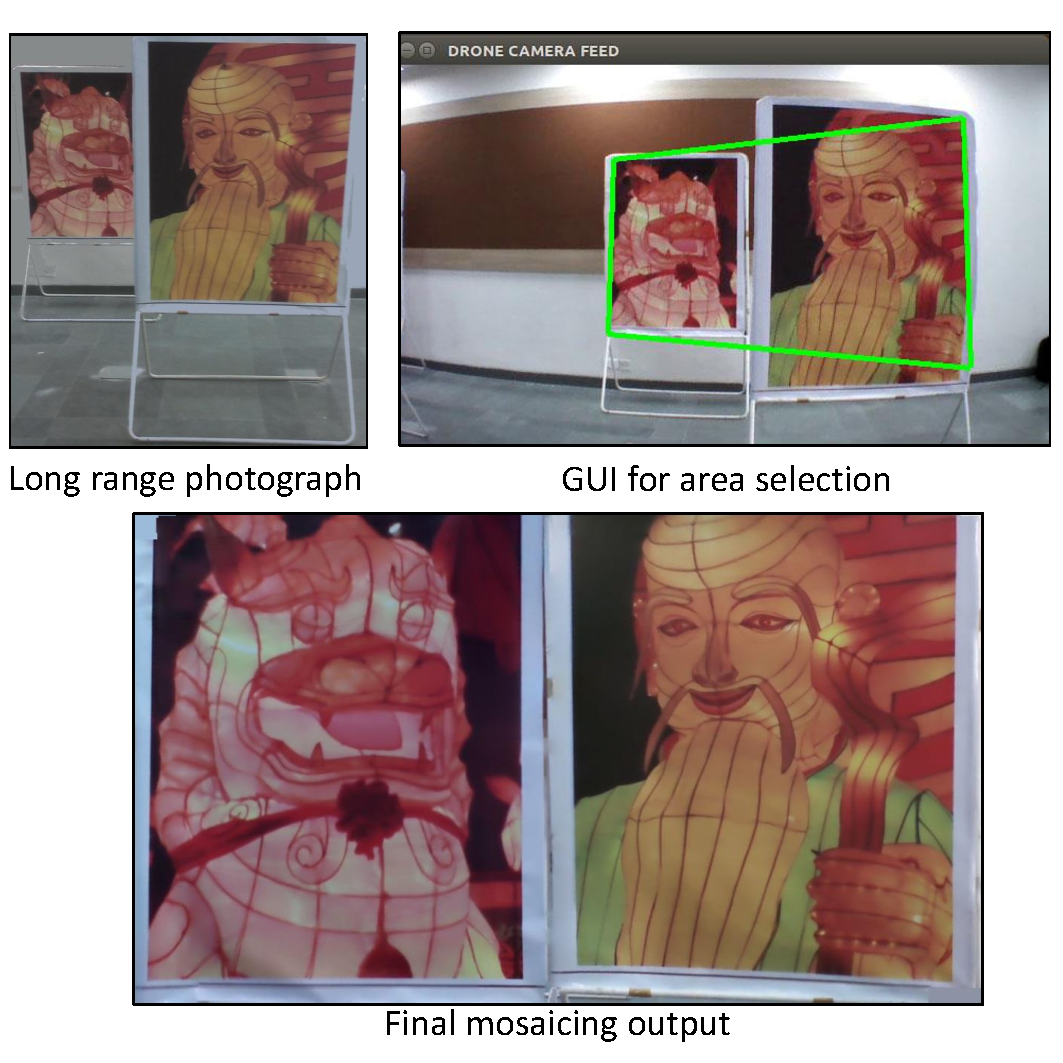
\includegraphics[width=0.9\textwidth]{figures/multiplanar/frontback.pdf}
\caption{There are two Chinese lanterns' exhibits, arranged parallel
to each other but having different depths as shown in the long-range
photograph(top-left). It is not possible to mosaic both of them in a single
panorama due to the difference in depths. We imaged those exhibits
independently through a quadcopter and brought the mosaic of the exhibit at larger
depth to the same depth of lesser depth exhibit mosaic. The final result is
shown in the bottom image.}
\label{fig:resultFrontBack}
\end{figure}

\section{Concluding remarks}
We have developed an end-to-end application for autonomously imaging multiplanar
regions using quadcopter. We have also developed an algorithm for `unrolling'
the multiplanar scene using the fusion of IMU data and video captured from
a quadcopter. Homography-based stitching cannot be used to create the mosaic of
scene spread over multiple planes. Also, using the handheld camera is cumbersome
to cover large multiplanar surfaces. Even with the UAVs manual control is very difficult.

In our solution, we autonomously maneuver a quadcopter along the planned path to
capture each plane in the multiplanar surface. The path planning for each plane
is done to estimate optimal locations such that images from the estimated
locations will cover the whole plane. Later, we stitch images for each plane to create a mini-panorama.
Finally, mini-panoramas are merged using positional information to form a full panorama.
Our method works in various setups like convex, concave as well as mixed.

%In the future, our method may be extended to cover any parametric surface in
%general.
It is practically impossible to image very large multiplanar surface using
just single quadcopter due to battery constraint. We can use multiple
quadcopters in collaboration to overcome this limitation. However, we need to
identify each quadcopter accurately to send proper commands. Identification of
a moving object in the unknown environment is a challenging task. Generally, 
fiducial markers are placed on an object for tracking. Motion blur introduced
due to swift movements of quadcopter causes problem in detection of current
fiducials. We discuss the design of motion blur resilient fiducials as well as
the detection of the same in next chapter.
